\documentclass[twoside]{book}

% Packages required by doxygen
\usepackage{calc}
\usepackage{doxygen}
\usepackage{graphicx}
\usepackage[utf8]{inputenc}
\usepackage{makeidx}
\usepackage{multicol}
\usepackage{multirow}
\usepackage{textcomp}
\usepackage[table]{xcolor}

% Font selection
\usepackage[T1]{fontenc}
\usepackage{mathptmx}
\usepackage[scaled=.90]{helvet}
\usepackage{courier}
\usepackage{amssymb}
\usepackage{sectsty}
\renewcommand{\familydefault}{\sfdefault}
\allsectionsfont{%
  \fontseries{bc}\selectfont%
  \color{darkgray}%
}
\renewcommand{\DoxyLabelFont}{%
  \fontseries{bc}\selectfont%
  \color{darkgray}%
}

% Page & text layout
\usepackage{geometry}
\geometry{%
  a4paper,%
  top=2.5cm,%
  bottom=2.5cm,%
  left=2.5cm,%
  right=2.5cm%
}
\tolerance=750
\hfuzz=15pt
\hbadness=750
\setlength{\emergencystretch}{15pt}
\setlength{\parindent}{0cm}
\setlength{\parskip}{0.2cm}
\makeatletter
\renewcommand{\paragraph}{%
  \@startsection{paragraph}{4}{0ex}{-1.0ex}{1.0ex}{%
    \normalfont\normalsize\bfseries\SS@parafont%
  }%
}
\renewcommand{\subparagraph}{%
  \@startsection{subparagraph}{5}{0ex}{-1.0ex}{1.0ex}{%
    \normalfont\normalsize\bfseries\SS@subparafont%
  }%
}
\makeatother

% Headers & footers
\usepackage{fancyhdr}
\pagestyle{fancyplain}
\fancyhead[LE]{\fancyplain{}{\bfseries\thepage}}
\fancyhead[CE]{\fancyplain{}{}}
\fancyhead[RE]{\fancyplain{}{\bfseries\leftmark}}
\fancyhead[LO]{\fancyplain{}{\bfseries\rightmark}}
\fancyhead[CO]{\fancyplain{}{}}
\fancyhead[RO]{\fancyplain{}{\bfseries\thepage}}
\fancyfoot[LE]{\fancyplain{}{}}
\fancyfoot[CE]{\fancyplain{}{}}
\fancyfoot[RE]{\fancyplain{}{\bfseries\scriptsize Generated on Sun Nov 3 2013 23\-:08\-:56 for Dflore22\-H\-W1 by Doxygen }}
\fancyfoot[LO]{\fancyplain{}{\bfseries\scriptsize Generated on Sun Nov 3 2013 23\-:08\-:56 for Dflore22\-H\-W1 by Doxygen }}
\fancyfoot[CO]{\fancyplain{}{}}
\fancyfoot[RO]{\fancyplain{}{}}
\renewcommand{\footrulewidth}{0.4pt}
\renewcommand{\chaptermark}[1]{%
  \markboth{#1}{}%
}
\renewcommand{\sectionmark}[1]{%
  \markright{\thesection\ #1}%
}

% Indices & bibliography
\usepackage{natbib}
\usepackage[titles]{tocloft}
\setcounter{tocdepth}{3}
\setcounter{secnumdepth}{5}
\makeindex

% Hyperlinks (required, but should be loaded last)
\usepackage{ifpdf}
\ifpdf
  \usepackage[pdftex,pagebackref=true]{hyperref}
\else
  \usepackage[ps2pdf,pagebackref=true]{hyperref}
\fi
\hypersetup{%
  colorlinks=true,%
  linkcolor=blue,%
  citecolor=blue,%
  unicode%
}

% Custom commands
\newcommand{\clearemptydoublepage}{%
  \newpage{\pagestyle{empty}\cleardoublepage}%
}


%===== C O N T E N T S =====

\begin{document}

% Titlepage & ToC
\hypersetup{pageanchor=false}
\pagenumbering{roman}
\begin{titlepage}
\vspace*{7cm}
\begin{center}%
{\Large Dflore22\-H\-W1 }\\
\vspace*{1cm}
{\large Generated by Doxygen 1.8.5}\\
\vspace*{0.5cm}
{\small Sun Nov 3 2013 23:08:56}\\
\end{center}
\end{titlepage}
\clearemptydoublepage
\tableofcontents
\clearemptydoublepage
\pagenumbering{arabic}
\hypersetup{pageanchor=true}

%--- Begin generated contents ---
\chapter{H\-W1}
\label{md__dropbox__curr__sem_cs340__h_w1__h_w1__r_e_a_d_m_e}
\hypertarget{md__dropbox__curr__sem_cs340__h_w1__h_w1__r_e_a_d_m_e}{}
\input{md__dropbox__curr__sem_cs340__h_w1__h_w1__r_e_a_d_m_e}
\chapter{Namespace Index}
\section{Namespace List}
Here is a list of all namespaces with brief descriptions\-:\begin{DoxyCompactList}
\item\contentsline{section}{\hyperlink{namespace_ui}{Ui} }{\pageref{namespace_ui}}{}
\end{DoxyCompactList}

\chapter{Hierarchical Index}
\section{Class Hierarchy}
This inheritance list is sorted roughly, but not completely, alphabetically\-:\begin{DoxyCompactList}
\item Q\-Main\-Window\begin{DoxyCompactList}
\item \contentsline{section}{Main\-Window}{\pageref{class_main_window}}{}
\end{DoxyCompactList}
\item \contentsline{section}{Ui\-\_\-\-Main\-Window}{\pageref{class_ui___main_window}}{}
\begin{DoxyCompactList}
\item \contentsline{section}{Ui\-:\-:Main\-Window}{\pageref{class_ui_1_1_main_window}}{}
\end{DoxyCompactList}
\end{DoxyCompactList}

\chapter{Class Index}
\section{Class List}
Here are the classes, structs, unions and interfaces with brief descriptions\-:\begin{DoxyCompactList}
\item\contentsline{section}{\hyperlink{class_main_window}{Main\-Window} \\*Main class \begin{DoxyVerb}   of my application for project CS340.\end{DoxyVerb}
 }{\pageref{class_main_window}}{}
\item\contentsline{section}{\hyperlink{class_ui_1_1_main_window}{Ui\-::\-Main\-Window} }{\pageref{class_ui_1_1_main_window}}{}
\item\contentsline{section}{\hyperlink{class_ui___main_window}{Ui\-\_\-\-Main\-Window} }{\pageref{class_ui___main_window}}{}
\end{DoxyCompactList}

\chapter{File Index}
\section{File List}
Here is a list of all files with brief descriptions\-:\begin{DoxyCompactList}
\item\contentsline{section}{Dropbox/\-Curr\-\_\-\-Sem/cs340/\-H\-W1/\-H\-W1/\hyperlink{main_8cpp}{main.\-cpp} }{\pageref{main_8cpp}}{}
\item\contentsline{section}{Dropbox/\-Curr\-\_\-\-Sem/cs340/\-H\-W1/\-H\-W1/\hyperlink{mainwindow_8cpp}{mainwindow.\-cpp} }{\pageref{mainwindow_8cpp}}{}
\item\contentsline{section}{Dropbox/\-Curr\-\_\-\-Sem/cs340/\-H\-W1/\-H\-W1/\hyperlink{mainwindow_8h}{mainwindow.\-h} }{\pageref{mainwindow_8h}}{}
\item\contentsline{section}{Dropbox/\-Curr\-\_\-\-Sem/cs340/\-H\-W1/\-H\-W1/\hyperlink{ui__mainwindow_8h}{ui\-\_\-mainwindow.\-h} }{\pageref{ui__mainwindow_8h}}{}
\end{DoxyCompactList}

\chapter{Namespace Documentation}
\hypertarget{namespace_ui}{\section{Ui Namespace Reference}
\label{namespace_ui}\index{Ui@{Ui}}
}
\subsection*{Classes}
\begin{DoxyCompactItemize}
\item 
class \hyperlink{class_ui_1_1_main_window}{Main\-Window}
\end{DoxyCompactItemize}


\subsection{Detailed Description}
$<$ 
\begin{DoxyCodeInclude}
\end{DoxyCodeInclude}
 
\chapter{Class Documentation}
\hypertarget{class_main_window}{\section{Main\-Window Class Reference}
\label{class_main_window}\index{Main\-Window@{Main\-Window}}
}


Main class \begin{DoxyVerb}   of my application for project CS340.\end{DoxyVerb}
.  




{\ttfamily \#include $<$mainwindow.\-h$>$}

Inheritance diagram for Main\-Window\-:\begin{figure}[H]
\begin{center}
\leavevmode
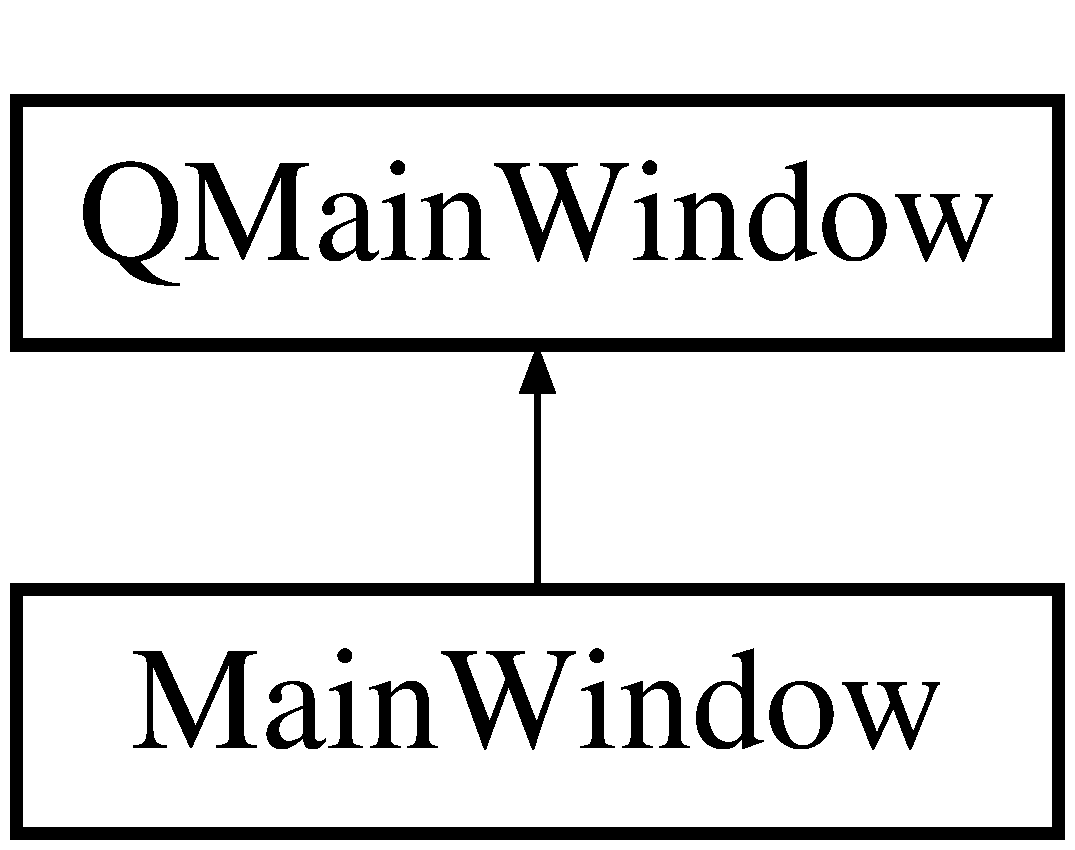
\includegraphics[height=2.000000cm]{class_main_window}
\end{center}
\end{figure}
\subsection*{Public Member Functions}
\begin{DoxyCompactItemize}
\item 
\hyperlink{class_main_window_a8b244be8b7b7db1b08de2a2acb9409db}{Main\-Window} (Q\-Widget $\ast$parent=0)
\begin{DoxyCompactList}\small\item\em \hyperlink{class_main_window}{Main\-Window} Class. \end{DoxyCompactList}\item 
\hyperlink{class_main_window_ae98d00a93bc118200eeef9f9bba1dba7}{$\sim$\-Main\-Window} ()
\end{DoxyCompactItemize}


\subsection{Detailed Description}
Main class \begin{DoxyVerb}   of my application for project CS340.\end{DoxyVerb}
. 

Inherits for Q\-Main\-Window from Qt 

Definition at line 26 of file mainwindow.\-h.



\subsection{Constructor \& Destructor Documentation}
\hypertarget{class_main_window_a8b244be8b7b7db1b08de2a2acb9409db}{\index{Main\-Window@{Main\-Window}!Main\-Window@{Main\-Window}}
\index{Main\-Window@{Main\-Window}!MainWindow@{Main\-Window}}
\subsubsection[{Main\-Window}]{\setlength{\rightskip}{0pt plus 5cm}Main\-Window\-::\-Main\-Window (
\begin{DoxyParamCaption}
\item[{Q\-Widget $\ast$}]{parent = {\ttfamily 0}}
\end{DoxyParamCaption}
)}}\label{class_main_window_a8b244be8b7b7db1b08de2a2acb9409db}


\hyperlink{class_main_window}{Main\-Window} Class. 

Constructor for \hyperlink{class_main_window}{Main\-Window}


\begin{DoxyParams}{Parameters}
{\em parent} & a parent widget, can be null\\
\hline
\end{DoxyParams}
This is where the underlying code to the user interface is. Any changes to the ui class are performed in this class. It also stores some of the information required for the window to display.

$<$ 
\begin{DoxyCodeInclude}
\end{DoxyCodeInclude}
 iostream library

$<$ 
\begin{DoxyCodeInclude}
\end{DoxyCodeInclude}
 mainwindow header file \hyperlink{class_main_window}{Main\-Window} class constructor\-This is where an instance of the ui class is created and any paramaters for the mainwindow class are initialized. 
\begin{DoxyParams}{Parameters}
{\em parent} & a parent widget, can be null \\
\hline
\end{DoxyParams}
$<$ int used in the window

$<$ int used in the window

$<$ int used in the window

$<$ int used in the window 

Definition at line 22 of file mainwindow.\-cpp.

\hypertarget{class_main_window_ae98d00a93bc118200eeef9f9bba1dba7}{\index{Main\-Window@{Main\-Window}!$\sim$\-Main\-Window@{$\sim$\-Main\-Window}}
\index{$\sim$\-Main\-Window@{$\sim$\-Main\-Window}!MainWindow@{Main\-Window}}
\subsubsection[{$\sim$\-Main\-Window}]{\setlength{\rightskip}{0pt plus 5cm}Main\-Window\-::$\sim$\-Main\-Window (
\begin{DoxyParamCaption}
{}
\end{DoxyParamCaption}
)}}\label{class_main_window_ae98d00a93bc118200eeef9f9bba1dba7}
\hyperlink{class_main_window}{Main\-Window} class destructor\-Deletes the instance of ui created in the constructor. $<$ delete ui instance 

Definition at line 38 of file mainwindow.\-cpp.



The documentation for this class was generated from the following files\-:\begin{DoxyCompactItemize}
\item 
Dropbox/\-Curr\-\_\-\-Sem/cs340/\-H\-W1/\-H\-W1/\hyperlink{mainwindow_8h}{mainwindow.\-h}\item 
Dropbox/\-Curr\-\_\-\-Sem/cs340/\-H\-W1/\-H\-W1/\hyperlink{mainwindow_8cpp}{mainwindow.\-cpp}\end{DoxyCompactItemize}

\hypertarget{class_ui_1_1_main_window}{\section{Ui\-:\-:Main\-Window Class Reference}
\label{class_ui_1_1_main_window}\index{Ui\-::\-Main\-Window@{Ui\-::\-Main\-Window}}
}


{\ttfamily \#include $<$ui\-\_\-mainwindow.\-h$>$}

Inheritance diagram for Ui\-:\-:Main\-Window\-:\begin{figure}[H]
\begin{center}
\leavevmode
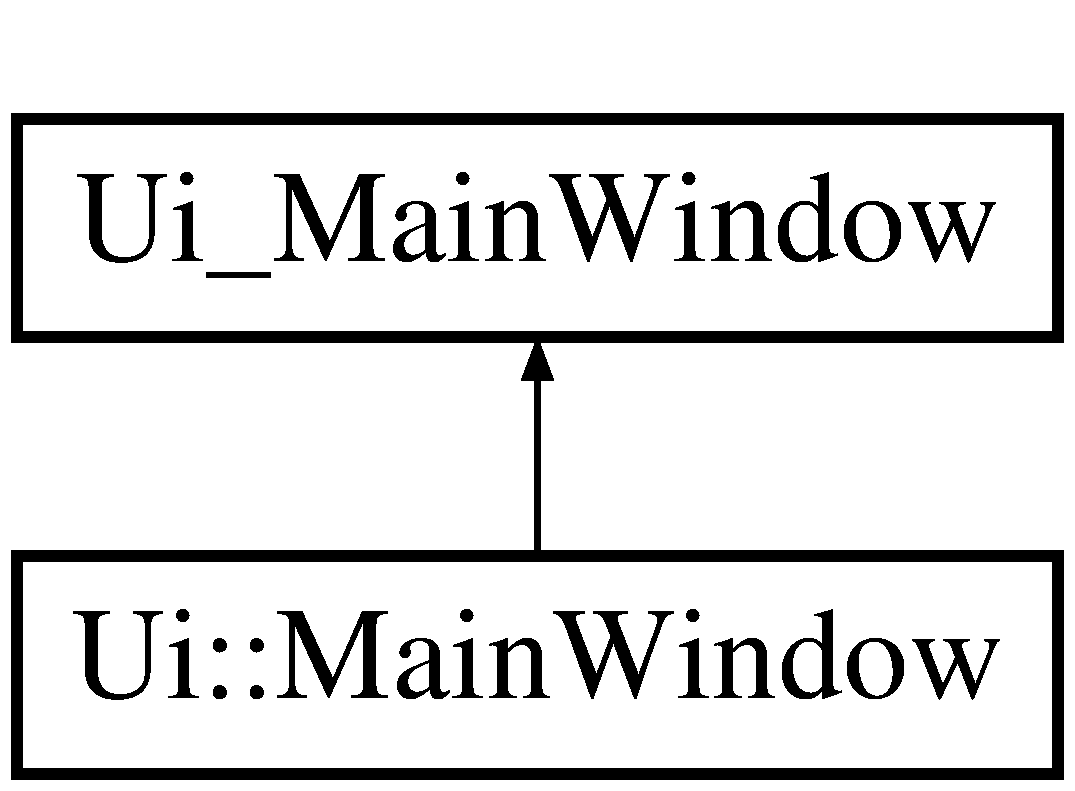
\includegraphics[height=2.000000cm]{class_ui_1_1_main_window}
\end{center}
\end{figure}
\subsection*{Additional Inherited Members}


\subsection{Detailed Description}


Definition at line 129 of file ui\-\_\-mainwindow.\-h.



The documentation for this class was generated from the following file\-:\begin{DoxyCompactItemize}
\item 
Dropbox/\-Curr\-\_\-\-Sem/cs340/\-H\-W1/\-H\-W1/\hyperlink{ui__mainwindow_8h}{ui\-\_\-mainwindow.\-h}\end{DoxyCompactItemize}

\hypertarget{class_ui___main_window}{\section{Ui\-\_\-\-Main\-Window Class Reference}
\label{class_ui___main_window}\index{Ui\-\_\-\-Main\-Window@{Ui\-\_\-\-Main\-Window}}
}


{\ttfamily \#include $<$ui\-\_\-mainwindow.\-h$>$}

Inheritance diagram for Ui\-\_\-\-Main\-Window\-:\begin{figure}[H]
\begin{center}
\leavevmode
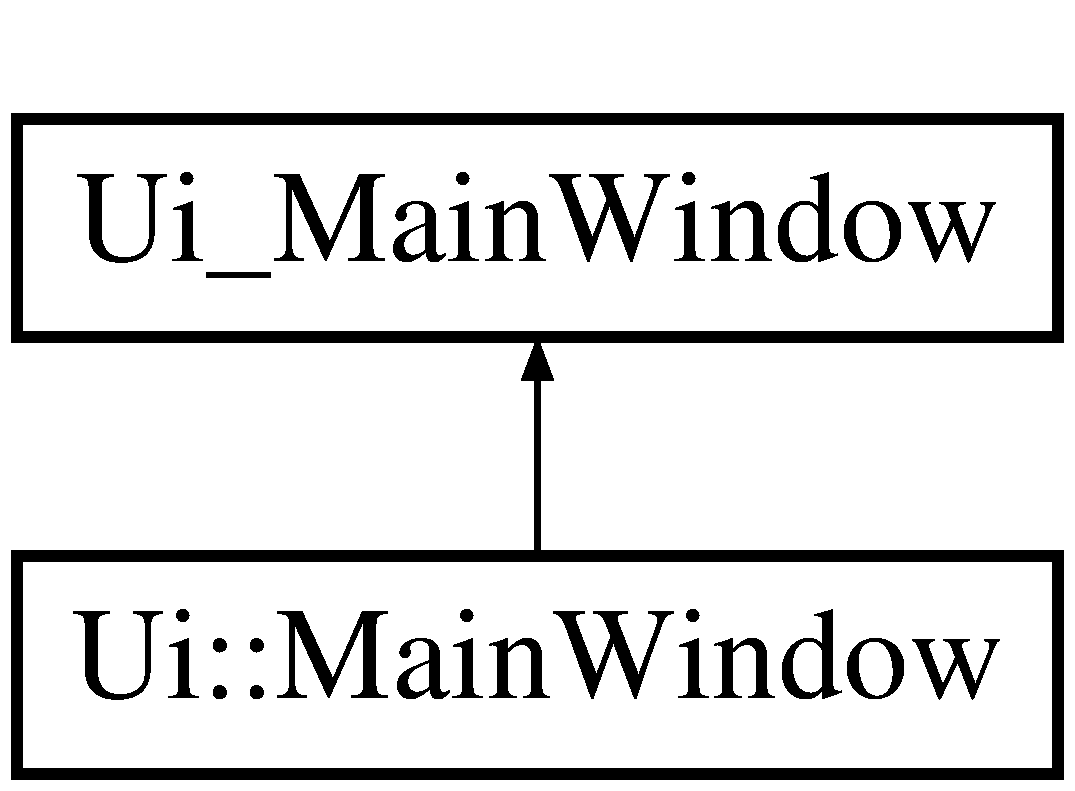
\includegraphics[height=2.000000cm]{class_ui___main_window}
\end{center}
\end{figure}
\subsection*{Public Member Functions}
\begin{DoxyCompactItemize}
\item 
void \hyperlink{class_ui___main_window_acf4a0872c4c77d8f43a2ec66ed849b58}{setup\-Ui} (Q\-Main\-Window $\ast$\hyperlink{class_main_window}{Main\-Window})
\item 
void \hyperlink{class_ui___main_window_a097dd160c3534a204904cb374412c618}{retranslate\-Ui} (Q\-Main\-Window $\ast$\hyperlink{class_main_window}{Main\-Window})
\end{DoxyCompactItemize}
\subsection*{Public Attributes}
\begin{DoxyCompactItemize}
\item 
Q\-Action $\ast$ \hyperlink{class_ui___main_window_a188c243f36a2dbc10e4e2a0ad94273b1}{action\-Quit}
\item 
Q\-Widget $\ast$ \hyperlink{class_ui___main_window_a30075506c2116c3ed4ff25e07ae75f81}{central\-Widget}
\item 
Q\-Push\-Button $\ast$ \hyperlink{class_ui___main_window_ad332d93084584930878f1daf5f84cdbf}{push\-Button}
\item 
Q\-Check\-Box $\ast$ \hyperlink{class_ui___main_window_ae8154204ed56489a091cf3a81af1f996}{check\-Box}
\item 
Q\-Check\-Box $\ast$ \hyperlink{class_ui___main_window_a42f54d4275ffecc52ea117a43a2a4def}{check\-Box\-\_\-2}
\item 
Q\-Check\-Box $\ast$ \hyperlink{class_ui___main_window_a7a0d575eebed36eac1592982b62ea449}{check\-Box\-\_\-3}
\item 
Q\-Dial $\ast$ \hyperlink{class_ui___main_window_a28c6790b1ca7f5d79927f26c7d7750ef}{Volume\-Control}
\item 
Q\-Progress\-Bar $\ast$ \hyperlink{class_ui___main_window_aebd7f3ec198128c31e8cd5c8ec4bc853}{Volume}
\item 
Q\-L\-C\-D\-Number $\ast$ \hyperlink{class_ui___main_window_aeaa664b636e02543a3047acb6d8918c5}{lcd\-Number}
\item 
Q\-Push\-Button $\ast$ \hyperlink{class_ui___main_window_a59a7d8124bce933d63f53f2153d447b4}{push\-Button\-\_\-2}
\item 
Q\-Plain\-Text\-Edit $\ast$ \hyperlink{class_ui___main_window_a6e290c2eca03b98b6f379c71910c0ed6}{plain\-Text\-Edit}
\item 
Q\-Status\-Bar $\ast$ \hyperlink{class_ui___main_window_a50fa481337604bcc8bf68de18ab16ecd}{status\-Bar}
\item 
Q\-Menu\-Bar $\ast$ \hyperlink{class_ui___main_window_a2be1c24ec9adfca18e1dcc951931457f}{menu\-Bar}
\item 
Q\-Menu $\ast$ \hyperlink{class_ui___main_window_a7ba84cb4cdd6a12dc83bf4e100bd8d80}{menu\-File}
\end{DoxyCompactItemize}


\subsection{Detailed Description}


Definition at line 31 of file ui\-\_\-mainwindow.\-h.



\subsection{Member Function Documentation}
\hypertarget{class_ui___main_window_a097dd160c3534a204904cb374412c618}{\index{Ui\-\_\-\-Main\-Window@{Ui\-\_\-\-Main\-Window}!retranslate\-Ui@{retranslate\-Ui}}
\index{retranslate\-Ui@{retranslate\-Ui}!Ui_MainWindow@{Ui\-\_\-\-Main\-Window}}
\subsubsection[{retranslate\-Ui}]{\setlength{\rightskip}{0pt plus 5cm}void Ui\-\_\-\-Main\-Window\-::retranslate\-Ui (
\begin{DoxyParamCaption}
\item[{Q\-Main\-Window $\ast$}]{Main\-Window}
\end{DoxyParamCaption}
)\hspace{0.3cm}{\ttfamily [inline]}}}\label{class_ui___main_window_a097dd160c3534a204904cb374412c618}


Definition at line 111 of file ui\-\_\-mainwindow.\-h.

\hypertarget{class_ui___main_window_acf4a0872c4c77d8f43a2ec66ed849b58}{\index{Ui\-\_\-\-Main\-Window@{Ui\-\_\-\-Main\-Window}!setup\-Ui@{setup\-Ui}}
\index{setup\-Ui@{setup\-Ui}!Ui_MainWindow@{Ui\-\_\-\-Main\-Window}}
\subsubsection[{setup\-Ui}]{\setlength{\rightskip}{0pt plus 5cm}void Ui\-\_\-\-Main\-Window\-::setup\-Ui (
\begin{DoxyParamCaption}
\item[{Q\-Main\-Window $\ast$}]{Main\-Window}
\end{DoxyParamCaption}
)\hspace{0.3cm}{\ttfamily [inline]}}}\label{class_ui___main_window_acf4a0872c4c77d8f43a2ec66ed849b58}


Definition at line 49 of file ui\-\_\-mainwindow.\-h.



\subsection{Member Data Documentation}
\hypertarget{class_ui___main_window_a188c243f36a2dbc10e4e2a0ad94273b1}{\index{Ui\-\_\-\-Main\-Window@{Ui\-\_\-\-Main\-Window}!action\-Quit@{action\-Quit}}
\index{action\-Quit@{action\-Quit}!Ui_MainWindow@{Ui\-\_\-\-Main\-Window}}
\subsubsection[{action\-Quit}]{\setlength{\rightskip}{0pt plus 5cm}Q\-Action$\ast$ Ui\-\_\-\-Main\-Window\-::action\-Quit}}\label{class_ui___main_window_a188c243f36a2dbc10e4e2a0ad94273b1}


Definition at line 34 of file ui\-\_\-mainwindow.\-h.

\hypertarget{class_ui___main_window_a30075506c2116c3ed4ff25e07ae75f81}{\index{Ui\-\_\-\-Main\-Window@{Ui\-\_\-\-Main\-Window}!central\-Widget@{central\-Widget}}
\index{central\-Widget@{central\-Widget}!Ui_MainWindow@{Ui\-\_\-\-Main\-Window}}
\subsubsection[{central\-Widget}]{\setlength{\rightskip}{0pt plus 5cm}Q\-Widget$\ast$ Ui\-\_\-\-Main\-Window\-::central\-Widget}}\label{class_ui___main_window_a30075506c2116c3ed4ff25e07ae75f81}


Definition at line 35 of file ui\-\_\-mainwindow.\-h.

\hypertarget{class_ui___main_window_ae8154204ed56489a091cf3a81af1f996}{\index{Ui\-\_\-\-Main\-Window@{Ui\-\_\-\-Main\-Window}!check\-Box@{check\-Box}}
\index{check\-Box@{check\-Box}!Ui_MainWindow@{Ui\-\_\-\-Main\-Window}}
\subsubsection[{check\-Box}]{\setlength{\rightskip}{0pt plus 5cm}Q\-Check\-Box$\ast$ Ui\-\_\-\-Main\-Window\-::check\-Box}}\label{class_ui___main_window_ae8154204ed56489a091cf3a81af1f996}


Definition at line 37 of file ui\-\_\-mainwindow.\-h.

\hypertarget{class_ui___main_window_a42f54d4275ffecc52ea117a43a2a4def}{\index{Ui\-\_\-\-Main\-Window@{Ui\-\_\-\-Main\-Window}!check\-Box\-\_\-2@{check\-Box\-\_\-2}}
\index{check\-Box\-\_\-2@{check\-Box\-\_\-2}!Ui_MainWindow@{Ui\-\_\-\-Main\-Window}}
\subsubsection[{check\-Box\-\_\-2}]{\setlength{\rightskip}{0pt plus 5cm}Q\-Check\-Box$\ast$ Ui\-\_\-\-Main\-Window\-::check\-Box\-\_\-2}}\label{class_ui___main_window_a42f54d4275ffecc52ea117a43a2a4def}


Definition at line 38 of file ui\-\_\-mainwindow.\-h.

\hypertarget{class_ui___main_window_a7a0d575eebed36eac1592982b62ea449}{\index{Ui\-\_\-\-Main\-Window@{Ui\-\_\-\-Main\-Window}!check\-Box\-\_\-3@{check\-Box\-\_\-3}}
\index{check\-Box\-\_\-3@{check\-Box\-\_\-3}!Ui_MainWindow@{Ui\-\_\-\-Main\-Window}}
\subsubsection[{check\-Box\-\_\-3}]{\setlength{\rightskip}{0pt plus 5cm}Q\-Check\-Box$\ast$ Ui\-\_\-\-Main\-Window\-::check\-Box\-\_\-3}}\label{class_ui___main_window_a7a0d575eebed36eac1592982b62ea449}


Definition at line 39 of file ui\-\_\-mainwindow.\-h.

\hypertarget{class_ui___main_window_aeaa664b636e02543a3047acb6d8918c5}{\index{Ui\-\_\-\-Main\-Window@{Ui\-\_\-\-Main\-Window}!lcd\-Number@{lcd\-Number}}
\index{lcd\-Number@{lcd\-Number}!Ui_MainWindow@{Ui\-\_\-\-Main\-Window}}
\subsubsection[{lcd\-Number}]{\setlength{\rightskip}{0pt plus 5cm}Q\-L\-C\-D\-Number$\ast$ Ui\-\_\-\-Main\-Window\-::lcd\-Number}}\label{class_ui___main_window_aeaa664b636e02543a3047acb6d8918c5}


Definition at line 42 of file ui\-\_\-mainwindow.\-h.

\hypertarget{class_ui___main_window_a2be1c24ec9adfca18e1dcc951931457f}{\index{Ui\-\_\-\-Main\-Window@{Ui\-\_\-\-Main\-Window}!menu\-Bar@{menu\-Bar}}
\index{menu\-Bar@{menu\-Bar}!Ui_MainWindow@{Ui\-\_\-\-Main\-Window}}
\subsubsection[{menu\-Bar}]{\setlength{\rightskip}{0pt plus 5cm}Q\-Menu\-Bar$\ast$ Ui\-\_\-\-Main\-Window\-::menu\-Bar}}\label{class_ui___main_window_a2be1c24ec9adfca18e1dcc951931457f}


Definition at line 46 of file ui\-\_\-mainwindow.\-h.

\hypertarget{class_ui___main_window_a7ba84cb4cdd6a12dc83bf4e100bd8d80}{\index{Ui\-\_\-\-Main\-Window@{Ui\-\_\-\-Main\-Window}!menu\-File@{menu\-File}}
\index{menu\-File@{menu\-File}!Ui_MainWindow@{Ui\-\_\-\-Main\-Window}}
\subsubsection[{menu\-File}]{\setlength{\rightskip}{0pt plus 5cm}Q\-Menu$\ast$ Ui\-\_\-\-Main\-Window\-::menu\-File}}\label{class_ui___main_window_a7ba84cb4cdd6a12dc83bf4e100bd8d80}


Definition at line 47 of file ui\-\_\-mainwindow.\-h.

\hypertarget{class_ui___main_window_a6e290c2eca03b98b6f379c71910c0ed6}{\index{Ui\-\_\-\-Main\-Window@{Ui\-\_\-\-Main\-Window}!plain\-Text\-Edit@{plain\-Text\-Edit}}
\index{plain\-Text\-Edit@{plain\-Text\-Edit}!Ui_MainWindow@{Ui\-\_\-\-Main\-Window}}
\subsubsection[{plain\-Text\-Edit}]{\setlength{\rightskip}{0pt plus 5cm}Q\-Plain\-Text\-Edit$\ast$ Ui\-\_\-\-Main\-Window\-::plain\-Text\-Edit}}\label{class_ui___main_window_a6e290c2eca03b98b6f379c71910c0ed6}


Definition at line 44 of file ui\-\_\-mainwindow.\-h.

\hypertarget{class_ui___main_window_ad332d93084584930878f1daf5f84cdbf}{\index{Ui\-\_\-\-Main\-Window@{Ui\-\_\-\-Main\-Window}!push\-Button@{push\-Button}}
\index{push\-Button@{push\-Button}!Ui_MainWindow@{Ui\-\_\-\-Main\-Window}}
\subsubsection[{push\-Button}]{\setlength{\rightskip}{0pt plus 5cm}Q\-Push\-Button$\ast$ Ui\-\_\-\-Main\-Window\-::push\-Button}}\label{class_ui___main_window_ad332d93084584930878f1daf5f84cdbf}


Definition at line 36 of file ui\-\_\-mainwindow.\-h.

\hypertarget{class_ui___main_window_a59a7d8124bce933d63f53f2153d447b4}{\index{Ui\-\_\-\-Main\-Window@{Ui\-\_\-\-Main\-Window}!push\-Button\-\_\-2@{push\-Button\-\_\-2}}
\index{push\-Button\-\_\-2@{push\-Button\-\_\-2}!Ui_MainWindow@{Ui\-\_\-\-Main\-Window}}
\subsubsection[{push\-Button\-\_\-2}]{\setlength{\rightskip}{0pt plus 5cm}Q\-Push\-Button$\ast$ Ui\-\_\-\-Main\-Window\-::push\-Button\-\_\-2}}\label{class_ui___main_window_a59a7d8124bce933d63f53f2153d447b4}


Definition at line 43 of file ui\-\_\-mainwindow.\-h.

\hypertarget{class_ui___main_window_a50fa481337604bcc8bf68de18ab16ecd}{\index{Ui\-\_\-\-Main\-Window@{Ui\-\_\-\-Main\-Window}!status\-Bar@{status\-Bar}}
\index{status\-Bar@{status\-Bar}!Ui_MainWindow@{Ui\-\_\-\-Main\-Window}}
\subsubsection[{status\-Bar}]{\setlength{\rightskip}{0pt plus 5cm}Q\-Status\-Bar$\ast$ Ui\-\_\-\-Main\-Window\-::status\-Bar}}\label{class_ui___main_window_a50fa481337604bcc8bf68de18ab16ecd}


Definition at line 45 of file ui\-\_\-mainwindow.\-h.

\hypertarget{class_ui___main_window_aebd7f3ec198128c31e8cd5c8ec4bc853}{\index{Ui\-\_\-\-Main\-Window@{Ui\-\_\-\-Main\-Window}!Volume@{Volume}}
\index{Volume@{Volume}!Ui_MainWindow@{Ui\-\_\-\-Main\-Window}}
\subsubsection[{Volume}]{\setlength{\rightskip}{0pt plus 5cm}Q\-Progress\-Bar$\ast$ Ui\-\_\-\-Main\-Window\-::\-Volume}}\label{class_ui___main_window_aebd7f3ec198128c31e8cd5c8ec4bc853}


Definition at line 41 of file ui\-\_\-mainwindow.\-h.

\hypertarget{class_ui___main_window_a28c6790b1ca7f5d79927f26c7d7750ef}{\index{Ui\-\_\-\-Main\-Window@{Ui\-\_\-\-Main\-Window}!Volume\-Control@{Volume\-Control}}
\index{Volume\-Control@{Volume\-Control}!Ui_MainWindow@{Ui\-\_\-\-Main\-Window}}
\subsubsection[{Volume\-Control}]{\setlength{\rightskip}{0pt plus 5cm}Q\-Dial$\ast$ Ui\-\_\-\-Main\-Window\-::\-Volume\-Control}}\label{class_ui___main_window_a28c6790b1ca7f5d79927f26c7d7750ef}


Definition at line 40 of file ui\-\_\-mainwindow.\-h.



The documentation for this class was generated from the following file\-:\begin{DoxyCompactItemize}
\item 
Dropbox/\-Curr\-\_\-\-Sem/cs340/\-H\-W1/\-H\-W1/\hyperlink{ui__mainwindow_8h}{ui\-\_\-mainwindow.\-h}\end{DoxyCompactItemize}

\chapter{File Documentation}
\hypertarget{main_8cpp}{\section{Dropbox/\-Curr\-\_\-\-Sem/cs340/\-H\-W1/\-H\-W1/main.cpp File Reference}
\label{main_8cpp}\index{Dropbox/\-Curr\-\_\-\-Sem/cs340/\-H\-W1/\-H\-W1/main.\-cpp@{Dropbox/\-Curr\-\_\-\-Sem/cs340/\-H\-W1/\-H\-W1/main.\-cpp}}
}
{\ttfamily \#include \char`\"{}mainwindow.\-h\char`\"{}}\\*
{\ttfamily \#include $<$Q\-Application$>$}\\*
\subsection*{Functions}
\begin{DoxyCompactItemize}
\item 
int \hyperlink{main_8cpp_a0ddf1224851353fc92bfbff6f499fa97}{main} (int argc, char $\ast$argv\mbox{[}$\,$\mbox{]})
\end{DoxyCompactItemize}


\subsection{Function Documentation}
\hypertarget{main_8cpp_a0ddf1224851353fc92bfbff6f499fa97}{\index{main.\-cpp@{main.\-cpp}!main@{main}}
\index{main@{main}!main.cpp@{main.\-cpp}}
\subsubsection[{main}]{\setlength{\rightskip}{0pt plus 5cm}int main (
\begin{DoxyParamCaption}
\item[{int}]{argc, }
\item[{char $\ast$}]{argv\mbox{[}$\,$\mbox{]}}
\end{DoxyParamCaption}
)}}\label{main_8cpp_a0ddf1224851353fc92bfbff6f499fa97}
Main class of the program\-This is where the main window class is called and then outputted. It will execute the Q\-T application

$<$ 
\begin{DoxyCodeInclude}
\end{DoxyCodeInclude}
 Q\-T app library $<$ create a Q\-T app

$<$ an instance of Main\-W\-Indow class

$<$ show the window class w

$<$ execute the Q\-T app 

Definition at line 11 of file main.\-cpp.


\hypertarget{mainwindow_8cpp}{\section{Dropbox/\-Curr\-\_\-\-Sem/cs340/\-H\-W1/\-H\-W1/mainwindow.cpp File Reference}
\label{mainwindow_8cpp}\index{Dropbox/\-Curr\-\_\-\-Sem/cs340/\-H\-W1/\-H\-W1/mainwindow.\-cpp@{Dropbox/\-Curr\-\_\-\-Sem/cs340/\-H\-W1/\-H\-W1/mainwindow.\-cpp}}
}
{\ttfamily \#include $<$iostream$>$}\\*
{\ttfamily \#include \char`\"{}mainwindow.\-h\char`\"{}}\\*
{\ttfamily \#include \char`\"{}ui\-\_\-mainwindow.\-h\char`\"{}}\\*

\hypertarget{mainwindow_8h}{\section{Dropbox/\-Curr\-\_\-\-Sem/cs340/\-H\-W1/\-H\-W1/mainwindow.h File Reference}
\label{mainwindow_8h}\index{Dropbox/\-Curr\-\_\-\-Sem/cs340/\-H\-W1/\-H\-W1/mainwindow.\-h@{Dropbox/\-Curr\-\_\-\-Sem/cs340/\-H\-W1/\-H\-W1/mainwindow.\-h}}
}
{\ttfamily \#include $<$Q\-Main\-Window$>$}\\*
\subsection*{Classes}
\begin{DoxyCompactItemize}
\item 
class \hyperlink{class_main_window}{Main\-Window}
\begin{DoxyCompactList}\small\item\em Main class \begin{DoxyVerb}   of my application for project CS340.\end{DoxyVerb}
. \end{DoxyCompactList}\end{DoxyCompactItemize}
\subsection*{Namespaces}
\begin{DoxyCompactItemize}
\item 
\hyperlink{namespace_ui}{Ui}
\end{DoxyCompactItemize}


\subsection{Detailed Description}
\begin{DoxyAuthor}{Author}
Luc Renambot 
\end{DoxyAuthor}
\begin{DoxyVersion}{Version}
1.\-0 
\end{DoxyVersion}
\hypertarget{mainwindow_8h_LICENSE}{}\subsection{L\-I\-C\-E\-N\-S\-E}\label{mainwindow_8h_LICENSE}
blah blah ? \hypertarget{mainwindow_8h_DESCRIPTION}{}\subsection{D\-E\-S\-C\-R\-I\-P\-T\-I\-O\-N}\label{mainwindow_8h_DESCRIPTION}
F\-O\-R T\-H\-E E\-M\-P\-E\-R\-O\-R!!!!!!!!!! 

Definition in file \hyperlink{mainwindow_8h_source}{mainwindow.\-h}.


\hypertarget{_r_e_a_d_m_e_8md}{\section{Dropbox/\-Curr\-\_\-\-Sem/cs340/\-H\-W1/\-H\-W1/\-R\-E\-A\-D\-M\-E.md File Reference}
\label{_r_e_a_d_m_e_8md}\index{Dropbox/\-Curr\-\_\-\-Sem/cs340/\-H\-W1/\-H\-W1/\-R\-E\-A\-D\-M\-E.\-md@{Dropbox/\-Curr\-\_\-\-Sem/cs340/\-H\-W1/\-H\-W1/\-R\-E\-A\-D\-M\-E.\-md}}
}

\hypertarget{ui__mainwindow_8h}{\section{Dropbox/\-Curr\-\_\-\-Sem/cs340/\-H\-W1/\-H\-W1/ui\-\_\-mainwindow.h File Reference}
\label{ui__mainwindow_8h}\index{Dropbox/\-Curr\-\_\-\-Sem/cs340/\-H\-W1/\-H\-W1/ui\-\_\-mainwindow.\-h@{Dropbox/\-Curr\-\_\-\-Sem/cs340/\-H\-W1/\-H\-W1/ui\-\_\-mainwindow.\-h}}
}
{\ttfamily \#include $<$Qt\-Core/\-Q\-Variant$>$}\\*
{\ttfamily \#include $<$Qt\-Widgets/\-Q\-Action$>$}\\*
{\ttfamily \#include $<$Qt\-Widgets/\-Q\-Application$>$}\\*
{\ttfamily \#include $<$Qt\-Widgets/\-Q\-Button\-Group$>$}\\*
{\ttfamily \#include $<$Qt\-Widgets/\-Q\-Check\-Box$>$}\\*
{\ttfamily \#include $<$Qt\-Widgets/\-Q\-Dial$>$}\\*
{\ttfamily \#include $<$Qt\-Widgets/\-Q\-Header\-View$>$}\\*
{\ttfamily \#include $<$Qt\-Widgets/\-Q\-L\-C\-D\-Number$>$}\\*
{\ttfamily \#include $<$Qt\-Widgets/\-Q\-Main\-Window$>$}\\*
{\ttfamily \#include $<$Qt\-Widgets/\-Q\-Menu$>$}\\*
{\ttfamily \#include $<$Qt\-Widgets/\-Q\-Menu\-Bar$>$}\\*
{\ttfamily \#include $<$Qt\-Widgets/\-Q\-Plain\-Text\-Edit$>$}\\*
{\ttfamily \#include $<$Qt\-Widgets/\-Q\-Progress\-Bar$>$}\\*
{\ttfamily \#include $<$Qt\-Widgets/\-Q\-Push\-Button$>$}\\*
{\ttfamily \#include $<$Qt\-Widgets/\-Q\-Status\-Bar$>$}\\*
{\ttfamily \#include $<$Qt\-Widgets/\-Q\-Widget$>$}\\*
\subsection*{Classes}
\begin{DoxyCompactItemize}
\item 
class \hyperlink{class_ui___main_window}{Ui\-\_\-\-Main\-Window}
\item 
class \hyperlink{class_ui_1_1_main_window}{Ui\-::\-Main\-Window}
\end{DoxyCompactItemize}
\subsection*{Namespaces}
\begin{DoxyCompactItemize}
\item 
\hyperlink{namespace_ui}{Ui}
\end{DoxyCompactItemize}

%--- End generated contents ---

% Index
\newpage
\phantomsection
\addcontentsline{toc}{part}{Index}
\printindex

\end{document}
